\section{Results: pretrained models and baselines}\label{sec:pretrained}

\subsection{Centered squares}

On aligned crops, the pretrained models lose identification accuracy without a collapse at small squares (Fig.~\ref{fig:squares}a). ArcFace R50 identifies \N{r1_arc_s00}\% of probes clean [\N{r1_arc_s00_lo}, \N{r1_arc_s00_hi}], \N{r1_arc_s05}\% with 5\% of the crop covered, \N{r1_arc_s10}\% at 10\%, \N{r1_arc_s20}\% at 20\%, \N{r1_arc_s30}\% at 30\%, and \N{r1_arc_s50}\% at 50\%; SFace identifies \N{r1_sf_s00}, \N{r1_sf_s05}, \N{r1_sf_s10}, \N{r1_sf_s20}, \N{r1_sf_s30}, and \N{r1_sf_s50}\%. ArcFace falls below 50\% between the 40\% and 50\% squares (\N{r1_arc_s40}\% and \N{r1_arc_s50}\%), SFace between 15\% and 20\% (\N{r1_sf_s15}\% and \N{r1_sf_s20}\%), and ArcFace scores higher than SFace in all \N{arc_gt_sf_n} conditions. From the 40\% square on, ``CNN, both'' scores above SFace (\N{r1_both_s40} against \N{r1_sf_s40}\% at 40\%). SFace is the only pretrained model in both the original runs and the study, and the crop, the alignment, the metric, and the protocol all changed between them, so the study does not isolate what any one change did. Crop coverage is also a different axis from the frame coverage of Section~\ref{sec:original}.

Raw crop pixels identify \N{r1_px_s00}\% clean, above chance (\N{chance}\%) and far below either pretrained model. The trained CNNs are discussed in Section~\ref{sec:ablation}; Fig.~\ref{fig:squares}b shows them on their own scale.

\begin{figure*}[t]
\centering
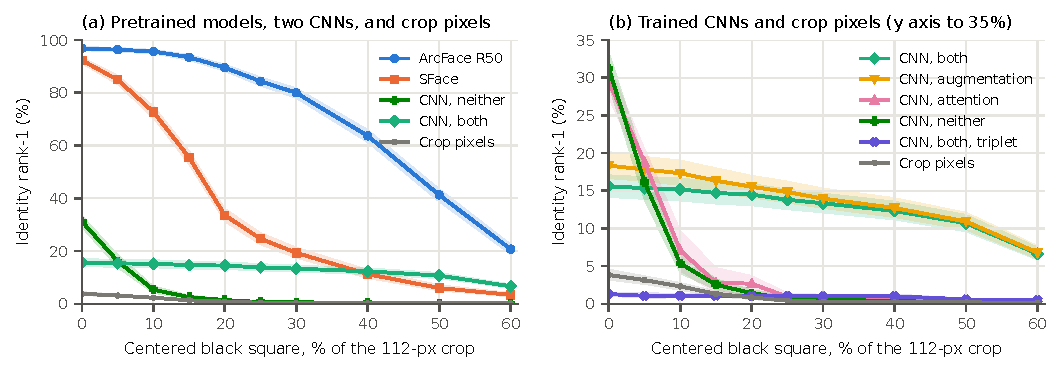
\includegraphics[width=\textwidth]{figures/fig_squares.pdf}
\caption{Identity rank-1 against the centered black square's share of the \N{crop}-pixel aligned crop, with 95\% bootstrap intervals (bands) over test identities and, for the trained CNNs, their \N{n_seeds} seeds. Chance is \N{chance}\%. (a) The pretrained models with two CNNs and raw pixels. (b) The five trained configurations and raw pixels, with the y axis to 35\%. ``Both'' = attention and occlusion augmentation.}
\label{fig:squares}
\end{figure*}

\subsection{Place and fill}

On these occluders, a band or an off-center square costs less than a centered square of similar or even smaller area (Fig.~\ref{fig:other}a): the 40\% lower band costs both models less than a centered 20\% square (ArcFace \N{r1_arc_low} against \N{r1_arc_s20}\%; SFace \N{r1_sf_low} against \N{r1_sf_s20}\%). Both bands cost far less than a centered square of similar area: ArcFace identifies \N{r1_arc_eye}\% with the eye band (\N{eye_area}\% of the crop) against \N{r1_arc_s25}\% with a 25\% square, and \N{r1_arc_low}\% with the lower band (\N{low_area}\%) against \N{r1_arc_s40}\% with a 40\% square; SFace \N{r1_sf_eye} against \N{r1_sf_s25}\%, and \N{r1_sf_low} against \N{r1_sf_s40}\%. A 20\% square at a random position costs less than a centered one (ArcFace \N{r1_arc_off20} against \N{r1_arc_s20}\%; SFace \N{r1_sf_off20} against \N{r1_sf_s20}\%). For SFace, the lower band costs less than the eye band; for ArcFace, it does not (\N{r1_arc_low} against \N{r1_arc_eye}\%). The centered square sits over the middle of the template, where the eyes and nose tip are (Fig.~\ref{fig:occluders}); the study does not test why place matters. The fill (black, gray, or noise) changes the pretrained models' rank-1 by less than \N{fill_max_pre_ub} points at the same area.

\begin{figure*}[t]
\centering
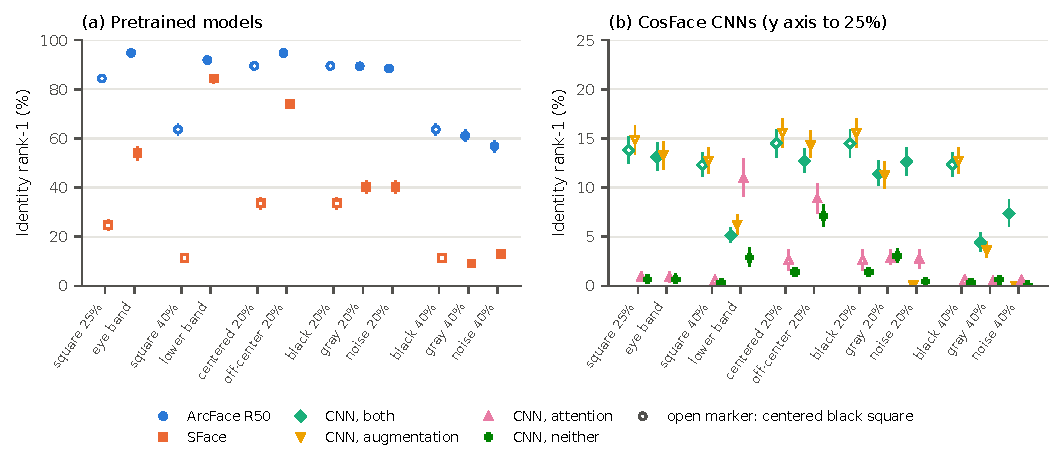
\includegraphics[width=\textwidth]{figures/fig_other.pdf}
\caption{Identity rank-1 for the occluders other than centered black squares (filled markers), each beside the centered black square of matched area (open markers), with 95\% bootstrap intervals. The eye band covers \N{eye_area}\% of the crop and is shown beside the 25\% square. (a) Pretrained models. (b) The four CosFace configurations, y axis to 25\% (the triplet runs, at \N{r1_tri_low} to \N{r1_tri_noise20}\%, are left out). ``CNN, augmentation'' has rank-1 at or below chance on both noise fills.}
\label{fig:other}
\end{figure*}

\subsection{Same image against identity}

The original protocol overstates identification for every model (Fig.~\ref{fig:gap}): in all \N{gap_n_all} model and square pairs up to 50\%, same-image rank-1 exceeds identity rank-1, by more than \N{gap_min_all_lb} points. For ArcFace, the gap is \N{gap_arc_s00} points [\N{gap_arc_s00_lo}, \N{gap_arc_s00_hi}] clean and \N{gap_arc_s50} at a 50\% square; for the four CosFace configurations, it is \N{gap_nn_s00} to \N{gap_both_s00} points clean, because, like every model, they match all clean images to themselves (a clean probe is its own gallery image) while identifying \N{cos_clean_lo} to \N{cos_clean_hi}\%.

The saved original model was trained for image matching and identifies poorly. On whole frames, it still matches \N{si_orig_f10}\% of images to themselves with 10\% of the frame covered, but identifies \N{r1_orig_f00}\% of clean probes [\N{r1_orig_f00_lo}, \N{r1_orig_f00_hi}], above chance and below raw frame pixels at \N{r1_pxf_f00}\% [\N{r1_pxf_f00_lo}, \N{r1_pxf_f00_hi}]. About 1 in \N{orig_overlap_share} of the frames it matches was probably in its training set (an estimate), which may raise its same-image numbers. Raw crop pixels show the same pattern: \N{si_px_s10}\% same-image against \N{r1_px_s10}\% identity at a 10\% square.

\begin{figure*}[t]
\centering
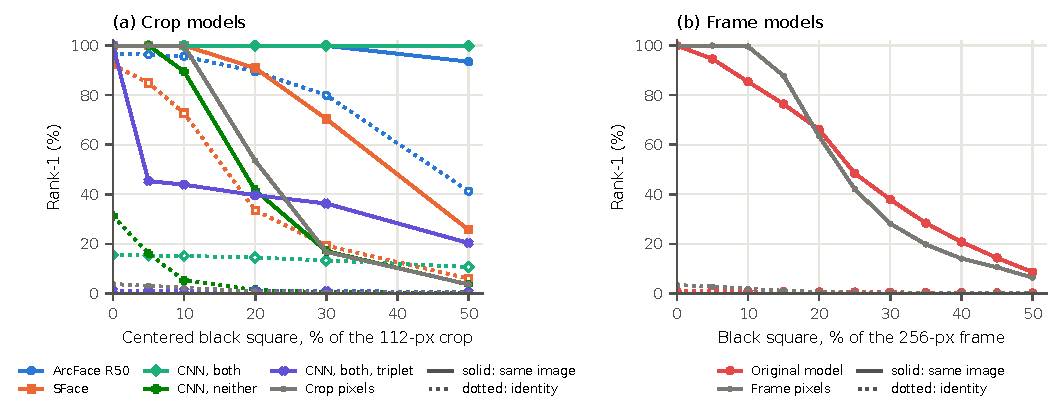
\includegraphics[width=\textwidth]{figures/fig_gap.pdf}
\caption{Same-image rank-1 (solid; the original protocol, each gallery image occluded and matched back) and identity rank-1 (dotted). (a) Six crop models, on the crop's coverage axis (``CNN, attention'' and ``CNN, augmentation'' are left out for legibility); ``CNN, both'' is at 100\% same-image at every square shown, so its line covers ArcFace's at the top through 30\%. (b) The frame-based arms on the frame's coverage axis, which is not comparable with (a). Same-image chance is also \N{chance}\%.}
\label{fig:gap}
\end{figure*}

\subsection{Verification at a fixed threshold}

For the pretrained models and the CosFace CNNs, at the FAR-\N{far1}\% threshold fixed on clean faces, occlusion lowers the mean false accept rate in every condition, and verification fails by rejecting genuine pairs (Table~\ref{tab:verif}). At the clean FAR-\N{far1}\% threshold, ArcFace's actual FAR falls to \N{far1_arc_s50}\% at a 50\% square and its TAR to \N{tarf1_arc_s50}\% [\N{tarf1_arc_s50_lo}, \N{tarf1_arc_s50_hi}]; a threshold re-set for that condition would report \N{tarpc1_arc_s50}\%. SFace's actual FAR falls to \N{far1_sf_s50}\% and its TAR to \N{tarf1_sf_s50}\% (re-set: \N{tarpc1_sf_s50}\%). Over every identity condition and seed, the actual FAR at the fixed \N{far1}\% threshold stays below \N{farmax1_cos_pre_ub}\% for the pretrained models and the CosFace configurations; it reaches \N{farmax1_tri}\% for the triplet runs and \N{farmax1_orig}\% for the original model at a \N{farmax1_orig_cond_pct}\% frame square. At the fixed \N{far01}\% threshold, the actual FAR of single CosFace seeds rises above \N{far01}\%, to as much as \N{farmax01_cos}\% (``CNN, attention'' at a 40\% square). The bands follow the identification results: SFace's fixed-threshold TAR is \N{tarf1_sf_eye}\% with the eye band and \N{tarf1_sf_low}\% with the lower band, and ArcFace's \N{tarf1_arc_eye}\% and \N{tarf1_arc_low}\%. The CosFace CNNs start far lower, at \N{tarf1_both_s00}\% clean for ``CNN, both'' and \N{tarf1_nn_s00}\% for ``CNN, neither''; the augmented network falls slowly with the square (\N{tarf1_both_s20}\% at 20\%, \N{tarf1_both_s50}\% at 50\%), while ``CNN, neither'' falls to \N{tarf1_nn_s20}\% at 20\%. With the face already aligned, the fixed-threshold TAR is the reading for a system that keeps one threshold across occluders; at the FAR-\N{far1}\% target, the re-set TAR is as high or higher under every occluder for these models.

\begin{table}[t]
\caption{Verification at a threshold fixed per model (per seed for the CNNs) on clean identity probes. TAR = true accept rate (\%) at the FAR-\N{far1}\% threshold, FAR = the actual false accept rate there (\%, mean over seeds), ``re-set'' = TAR with the threshold set on that condition's own impostors, TAR$_{0.1}$ = TAR at the fixed FAR-\N{far01}\% threshold. Trained CNNs are means of \N{n_seeds} seeds.}
\label{tab:verif}
\centering\small
\setlength{\tabcolsep}{3.5pt}
% Generated by make_numbers.py. Do not edit.
\begin{tabular}{@{}llrrrr@{}}
\toprule
Model & Condition & TAR & FAR & TAR, re-set & TAR$_{0.1}$ \\
\midrule
ArcFace R50 & clean & 97.5 & 1.00 & 97.5 & 97.0 \\
 & square 20\% & 95.1 & 0.69 & 95.8 & 89.4 \\
 & square 50\% & 57.3 & 0.36 & 67.9 & 28.4 \\
 & eye band & 97.1 & 0.90 & 97.1 & 95.7 \\
 & lower band & 95.3 & 0.66 & 95.8 & 91.8 \\
\addlinespace
SFace & clean & 95.7 & 1.00 & 95.7 & 92.8 \\
 & square 20\% & 53.9 & 0.62 & 59.3 & 28.0 \\
 & square 50\% & 4.5 & 0.12 & 17.9 & 0.8 \\
 & eye band & 69.1 & 0.43 & 75.9 & 45.9 \\
 & lower band & 88.9 & 0.30 & 92.4 & 80.2 \\
\addlinespace
CNN, both & clean & 36.7 & 1.00 & 36.7 & 17.8 \\
 & square 20\% & 34.5 & 0.97 & 34.8 & 16.1 \\
 & square 50\% & 26.7 & 0.85 & 28.3 & 10.8 \\
\addlinespace
CNN, neither & clean & 55.1 & 1.00 & 55.1 & 34.2 \\
 & square 20\% & 4.6 & 0.43 & 7.8 & 0.6 \\
 & square 50\% & 0.6 & 0.28 & 2.1 & 0.0 \\
\bottomrule
\end{tabular}

\end{table}
